\documentclass{article}
\usepackage[a4paper, left=0.5in, right=0.5in, top=1.in, bottom=1.5in]{geometry}
\usepackage{indentfirst}
\usepackage{graphicx}
\usepackage{float}
\usepackage{minted}
% \usepackage{cite}
\usepackage{hyperref}
\usepackage[english]{babel}
\usepackage{amsmath}
\usepackage{amssymb}
\usepackage{commath}

\title{\textbf{Bayer's Pattern}}
\author{\textbf{Narendiran S}}
\date{\textbf{06-06-2020}}

\begin{document}
\Large
\maketitle

\section{Use Case}

A Bayer filter mosaic is a color filter array (CFA) for arranging RGB color filters on a square grid of photosensors.
Its particular arrangement of color filters is used in most single-chip digital image sensors used in digital cameras, camcorders, and scanners to create a color image.
The filter pattern is half green, one quarter red and one quarter blue.

\begin{figure}[H]
    \centering
    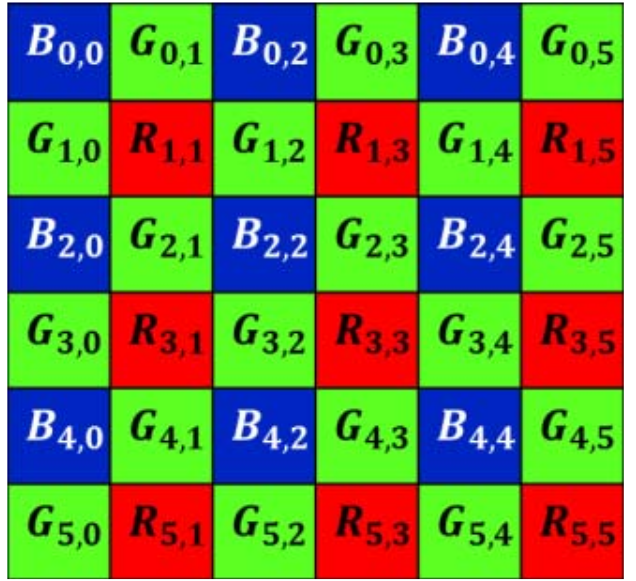
\includegraphics[scale=0.3]{DocResources/BayersPattern.png}
    \caption{Bayer Pattern}
\end{figure}

\section{Creation of Bayer Pattern Image in PYthon}
\begin{minted}[frame=lines, breaklines, linenos]{python}
bayerImg = np.zeros((actualImg.shape[0], actualImg.shape[1]), dtype=np.uint8)

# Blue values - odd rows and odd columns
bayerImg[::2, ::2] = actualImg[::2, ::2, 2]
bayerImg2[::2, ::2, 2] = actualImg[::2, ::2, 2]

# Red values - even rows and even columns
bayerImg[1::2, 1::2] = actualImg[1::2, 1::2, 0]
bayerImg2[1::2, 1::2, 0] = actualImg[1::2, 1::2, 0]

# Green values - BGBGBG....
bayerImg[1::2, ::2] = actualImg[1::2, ::2, 1]
bayerImg2[1::2, ::2, 1] = actualImg[1::2, ::2, 1]

# Green values - GRGRGR....
bayerImg[::2, 1::2] = actualImg[::2, 1::2, 1]
bayerImg2[::2, 1::2, 1] = actualImg[::2, 1::2, 1]
\end{minted}

\section{Example}
\begin{figure}[H]
    \begin{center}
        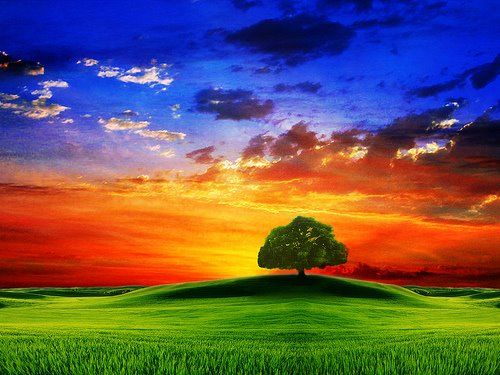
\includegraphics[scale=0.5]{originalImage.jpg}
        \caption{Original Image}
    \end{center}
\end{figure}

\begin{figure}[H]
    \begin{center}
        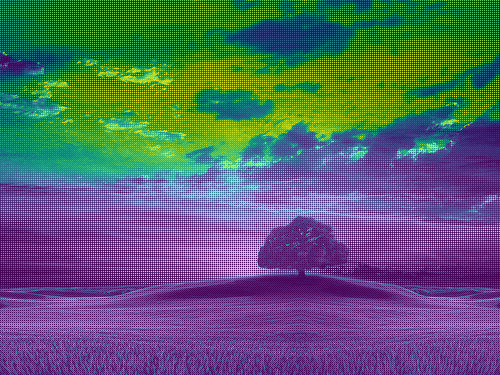
\includegraphics[scale=0.7]{DocResources/BayerImage_SingleChannel.png}
        \caption{Bayer Image with just one channel}
    \end{center}
\end{figure}

\begin{figure}[H]
    \begin{center}
        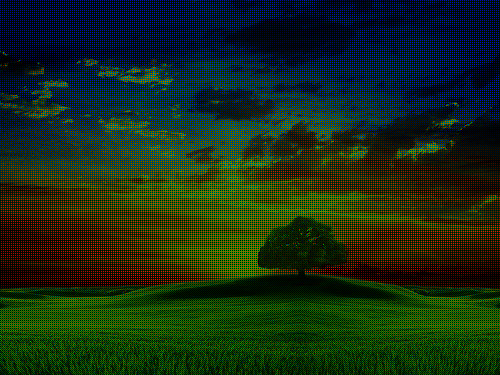
\includegraphics[scale=0.7]{DocResources/BayerImage_3Channel.png}
        \caption{Bayer Image with a 3 channel (zeros at other positions)}
    \end{center}
\end{figure}


\section{Implementations}
Used this paper\cite{papera} for Implementations.
Two Implementation were done: VivadoProject/project\_1 -- without padding of zeros - so we get reduced resolution. VivadoProject/ReconstructionWithPadding -- with Padding of zeros - to get same resolution.
The block diagram can be seen below:
\begin{figure}[H]
    \centering
    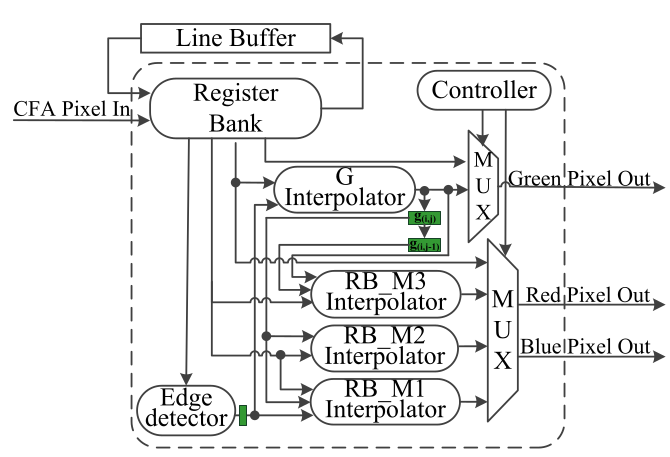
\includegraphics[scale=0.5]{DocResources/BlockDiagram.png}
\end{figure}

\begin{itemize}
    \item THe Register Bank (uses line buffers) producess a 3x5 pixel grid.
    \item This value is gien to Edge Detector to get DH and DV.
    \item The these values are given to Ginterpolator to get G values.
    \item The these values are given to RBM1 to get RB when the current pixel is Blue or Red.
    \item The these values are given to RBM2 to get RB when the current pixel is Green (BGBG.. pattern).
    \item The these values are given to RBM3 to get RB when the current pixel is Green (GRGR.. pattern).
\end{itemize}

\subsection{Line Buffers}
Line Buffers holds the values of a complete Row of an Image.
The length of line buffer is equal to the width of the Image.
These Line buffers are made from shift registers.

\subsection{Register Banks}
They are obtained from Line Buffers.
Here 3 Line Buffers are used connected serially as shown below:

\begin{figure}[H]
    \centering
    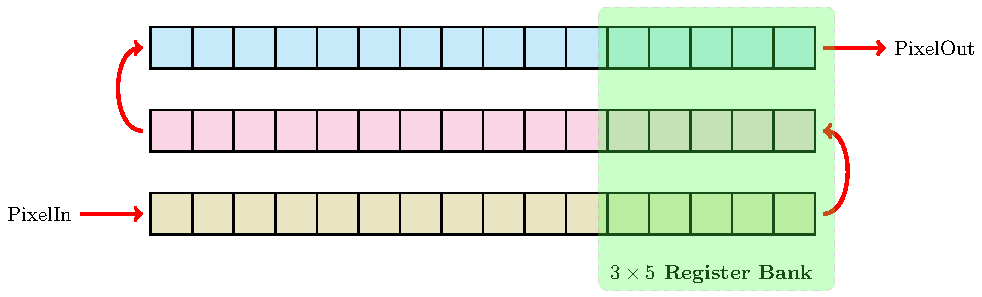
\includegraphics[scale=0.8]{DocResources/RegisterBankCreation.pdf}
\end{figure}


\subsection{EdgeDetector}
\begin{align}
    DV_{i,j} & = \abs{P_{i-1, j-1} - P_{i+1,j-1}} + \abs{P_{i-1, j} - P_{i+1,j}} + \abs{P_{i-1, j+1} - P_{i+1,j+1}} \\
    DH_{i,j} & = \abs{P_{i+1, j+1} - P_{i+1,j-1}} + \abs{P_{i, j+1} - P_{i,j-1}} + \abs{P_{i-1, j+1} - P_{i-1,j-1}}
\end{align}
For absoluted differnce - found which is greater and subtracted the lesser value from the greater value.

\subsection{G Interpolator}
Finding Green when the current pixel is Blue or Red.


The equations can be seen below and their representations can be seen in the figure.
    {
        \small
        \begin{equation}
            G_{i,j} = \begin{cases}
                \frac{1}{8}(P_{i-1,j} + P_{i+1,j}) + \frac{3}{8}(P_{i,j-1} + P_{i,j+1}) - \frac{1}{4}(P_{i,j-2} + P_{i,j+2}) + \frac{1}{2}P_{i,j}, & \text{DH} = {DV} \\
                \frac{1}{2}(P_{i,j-1} + P_{i,j+1}) - \frac{1}{4}(P_{i,j-2} + P_{i,j+2}) + \frac{1}{2}P_{i,j},                                      & \text{DH} < {DV} \\
                \frac{3}{8}(P_{i-1,j} + P_{i+1,j}) + \frac{1}{8}(P_{i,j-1} + P_{i,j+1}) - \frac{1}{8}(P_{i,j-2} + P_{i,j+2}) + \frac{1}{4}P_{i,j}, & \text{DH} > {DV} \\
            \end{cases}
        \end{equation}
    }
\begin{figure}[H]
    \centering
    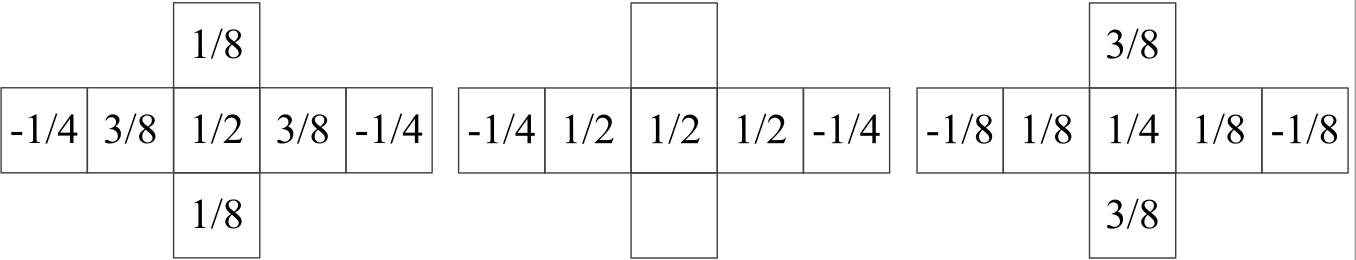
\includegraphics[scale=0.3]{DocResources/Gint.png}
\end{figure}

The pixel values are added an shifted and added.

\subsection{RB Interpolator - M1}
Finding Red or Blue when the current pixel is Blue or Red.

The equations can be seen below and their representations can be seen in the figure.
    {
        \small
        \begin{equation}
            RBM1_{i,j} = \begin{cases}
                \frac{1}{4}(P_{i-1,j-1} + P_{i+1,j-1} + P_{i+1,j-1} + P_{i+1,j+1}) - \frac{1}{4}(P_{i-1,j} + P_{i,j-1} + P_{i,j+1} + P_{i+1,j}) + g_{i,j} ,             & \text{DH} = {DV} \\
                \frac{1}{4}(P_{i-1,j-1} + P_{i+1,j-1} + P_{i+1,j-1} + P_{i+1,j+1}) - \frac{3}{8}(P_{i-1,j} + P_{i+1,j}) - \frac{1}{8}(P_{i,j-1} + P_{i,j+1}) + g_{i,j}, & \text{DH} > {DV} \\
                \frac{1}{4}(P_{i-1,j-1} + P_{i+1,j-1} + P_{i+1,j-1} + P_{i+1,j+1}) - \frac{1}{8}(P_{i-1,j} + P_{i+1,j}) - \frac{3}{8}(P_{i,j-1} + P_{i,j+1}) + g_{i,j}, & \text{DH} < {DV} \\
            \end{cases}
        \end{equation}
    }

$g_{i,j}$ is the updated G interpolated value.

\begin{figure}[H]
    \centering
    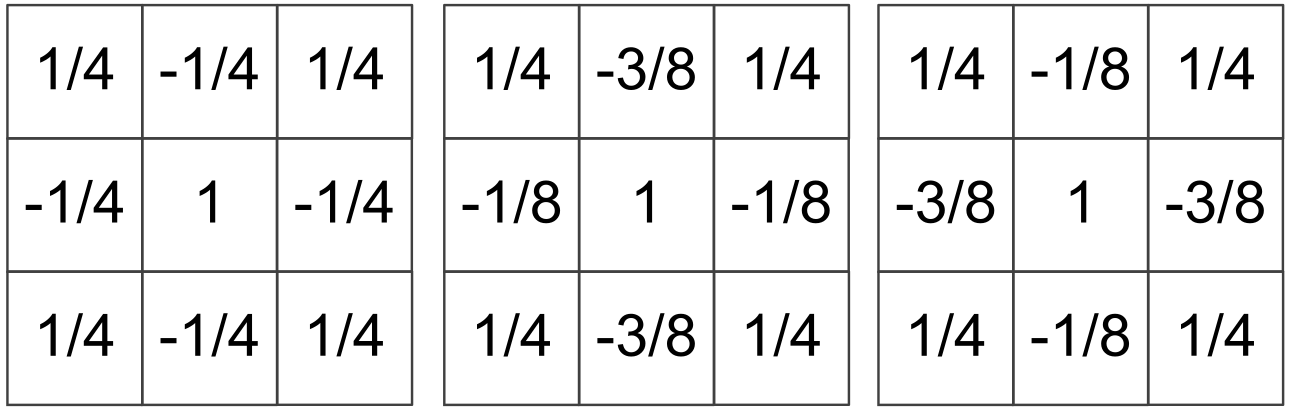
\includegraphics[scale=0.3]{DocResources/RBM1.png}
\end{figure}





\subsection{RB Interpolator - M2}
Finding Red or Blue when the current pixel is Green (either BGBG... or GRGR...).

The equations can be seen below and their representations can be seen in the figure.
    {
        \begin{equation}
            RBM2_{i,j} = \frac{1}{2}(P_{i-1,j} + P_{i+1,j}) - \frac{1}{8}(P_{i-1,j-1} + P_{i+1,j-1} + P_{i+1,j-1} + P_{i+1,j+1}) + \frac{1}{2}P_{i,j}
        \end{equation}
    }


\begin{figure}[H]
    \centering
    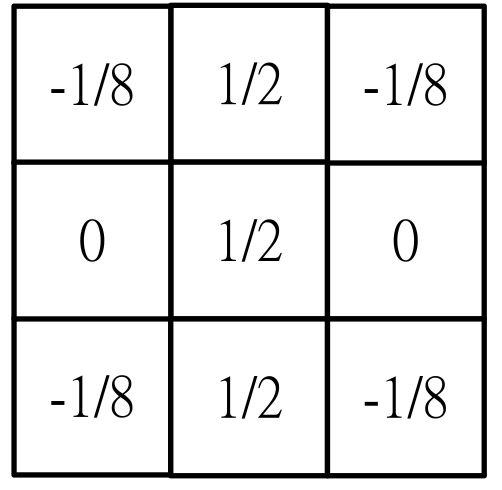
\includegraphics[scale=0.3]{DocResources/RBM2.png}
\end{figure}


\subsection{RB Interpolator - M3}
Finding Red or Blue when the current pixel is Green (either BGBG... or GRGR...).

The equations can be seen below and their representations can be seen in the figure.
    {
        \begin{equation}
            RBM3_{i,j} = \frac{1}{2}(P_{i,j-1} + P_{i,j+1})
        \end{equation}
    }



\begin{thebibliography}{9}
    \bibitem{papera}
    S. Chen and E. Ma, "VLSI Implementation of an Adaptive Edge-Enhanced Color Interpolation Processor for Real-Time Video Applications," in IEEE Transactions on Circuits and Systems for Video Technology, vol. 24, no. 11, pp. 1982-1991, Nov. 2014, doi: 10.1109/TCSVT.2014.2317890.

\end{thebibliography}

\end{document}
